\documentclass{article}

\usepackage{../../Style}

\title{Toric varieties}
\author{Shing Tak Lam}
\date{Lent 2023\footnote{Based on lectures by Renata Picciotto. Last updated \today.}}

\makeindex

\begin{document}

\maketitle

\tableofcontents

\lec

In this course, we do everything over \(\C\).

\section{What is a toric variety?}

\begin{definition}
    [affine variety] An \emph{affine variety}\index{affine variety} is \(V = \Spec(R)\), where \(R\) is a finitely generated integral\footnote{\(R\) is an integral domain.} \(\C\)-algebra.
\end{definition}

\underline{Fact:} Given such an \(R\), we can choose generators and relations, and write
\[R = \frac{\C[x_1, \dots, x_n]}{I}\]
where \(I\) is a prime ideal. This gives an affine embedding. i.e. a closed embedding
\[V = \van(I) = \A^n\]
Note that the affine embedding is not unique.

\begin{definition}
    [(complex) variety] A \emph{(complex) variety}\index{variety} is a scheme \(X\) which is integral (reduced and irreducible), separated, and of finite type.
\end{definition}

We can avoid schemes, and glue varieties out of affine varieties. We need 
\begin{enumerate}
    \item a finite collection \(\{V_\alpha\}_{\alpha \in A}\) of affine varieties, say \(V_\alpha = \Spec(R_\alpha)\), 
    \item for \(\alpha, \beta \in A\), we need Zariski opens \(V_{\alpha\beta} \sse V_\alpha\),
    \item algebraic transition maps \(g_{\alpha\beta} : V_{\alpha\beta} \to V_{\beta\alpha}\), satisfying the usual cocycle conditions,
    \item check that the resulting
    \[X = \frac{\bigsqcup_\alpha V_\alpha}{\sim}\]
    is irreducible and separated (Hausdorff).
\end{enumerate}

\begin{definition}
    [torus] An \emph{(algebraic complex) torus of dimension \(n\)}\index{torus} is 
    \[\T^n = (\C^*)^n = \Spec(\C[x_1^{\pm 1}, \dots, x_n^{\pm 1}]) = (\A^1 \setminus \{0\})^n\]
\end{definition}

Note that this is not the same as the usual torus \((S^1)^n\). In particular, we have an affine embedding
\[\T^n = \Spec\left(\frac{\C[z_0, \dots, z_n]}{\inner{z_0\cdots z_n - 1}}\right) = \van(z_0\cdots z_n - 1) \sse \A^{n+1}\]
\underline{Exercise:} Check that we have an isomorphism of rings
\[\C[z_1^{\pm 1}, \dots, z_n^{\pm 1}] \cong \frac{\C[z_0, \dots, z_n]}{\inner{z_0\cdots z_n - 1}}\]

The torus is also a \emph{commutative group scheme}\index{commutative group scheme}, that is, we have algebraic morphisms
\begin{align*}
    e : \bullet &\to \T^n \\
    m : \T^n \times \T^n &\to \T^n \\
    i : \T^n &\to \T^n
\end{align*}
making \(\T^n\) into an abelian group with identity \(e\), multiplication \(m\) and inverse \(i\). On the level of coordinate rings, we have the \emph{identity section},
\begin{align*}
    e^\sharp : \C[t_1^{\pm 1}, \dots, t_n^{\pm 1}] &\to \C \\
    t_i^{\pm 1} &\mapsto 1
\end{align*}
The multiplication map is given by pointwise operations, i.e.
\[m((x_1, \dots, x_n), (y_1, \dots, y_n)) = (x_1y_1, \dots, x_ny_n)\]
With this, we have \emph{comultiplication}
\begin{align*}
    m^\sharp : \C[t_1^{\pm 1}, \dots, t_n^{\pm 1}] &\to \C[x_1^{\pm 1}, \dots, x_n^{\pm 1}] \otimes \C[y_1^{\pm 1}, \dots, y_n^{\pm 1}] \\
    t_i &\mapsto x_i \otimes y_i
\end{align*}
and the inverse map is given by
\begin{align*}
    i^\sharp : \C[t_1^{\pm 1}, \dots, t_n^{\pm 1}] &\to \C[t_1^{\pm 1}, \dots, t_n^{\pm 1}] \\
    t_i &\mapsto t_i^{-1}
\end{align*}

\begin{definition}
    [toric variety] A \emph{toric variety}\index{toric variety} is a variety \(X\) with a dense open \(\T^n \sse X\), and an action (i.e. algebraic map)
    \[a : \T^n \times X \to X\]
    which extends the multiplication on \(X\).
\end{definition}

\begin{example}
    \(\T^n\) is itself a toric variety.
\end{example}
Cohomology
\begin{example}
    \(\A^n = \Spec(\C[x_1, \dots, x_n])\), with the torus
    \[\Spec(\C[x_1^{\pm 1}, \dots, x_n^{\pm 1}])\]
    with
    \[a((t_1, \dots, t_n), (x_1, \dots, x_n)) = (t_1x_1, \dots, t_nx_n)\]
\end{example}

\begin{example}
    Projective space
    \[\P^n = \Proj(\C[z_0, \dots, z_n]) = \{(z_0 : \dots : z_n) \mid (z_0, \dots, z_n) \ne (0, \dots, 0)\}\]
    is also a toric variety, with torus
    \[\T^n = \{(z_0 : \dots : z_n) \mid z_0\cdots z_n = 1\}\]
    with action given coordinate-wise again, i.e.
    \[a((t_0: \dots: t_n), (z_0:\dots:z_n)) = (t_0z_0:\dots:t_nz_n)\]
    in non-homogeneous coordinates (i.e. in the affine \(z_0 \ne 0\)) of the torus, we can define the action by
    \[(t_1, \dots, t_n) \cdot (z_0:\dots : z_n) = (z_0 : t_1z_1: \dots : t_nz_n)\]
    We can check that \(\T^n\) is contained in all of the standard opens \(U_i = D(z_i)\), and if we choose the usual affine coordinates, then \(\T^n\) embeds into affine space as above.
\end{example}

Toric varieties are determined by the dimension \(n\) of the torus, and the \emph{toric boundary}\index{toric boundary} \(X \setminus \T^n\). For example, \(\P^2 \setminus \T^2\) has three components,
\begin{enumerate}
    \item \(V_0 = \van(z_0)\),
    \item \(V_1 = \van(z_1)\),
    \item \(V_2 = \van(z_2)\)
\end{enumerate}
The \(V_i\) intersect pairwise, but not all three at the same time. Each \(V_i\) is invariant under the action of the torus, so \(\P^2\) can be represented as

\begin{center}
    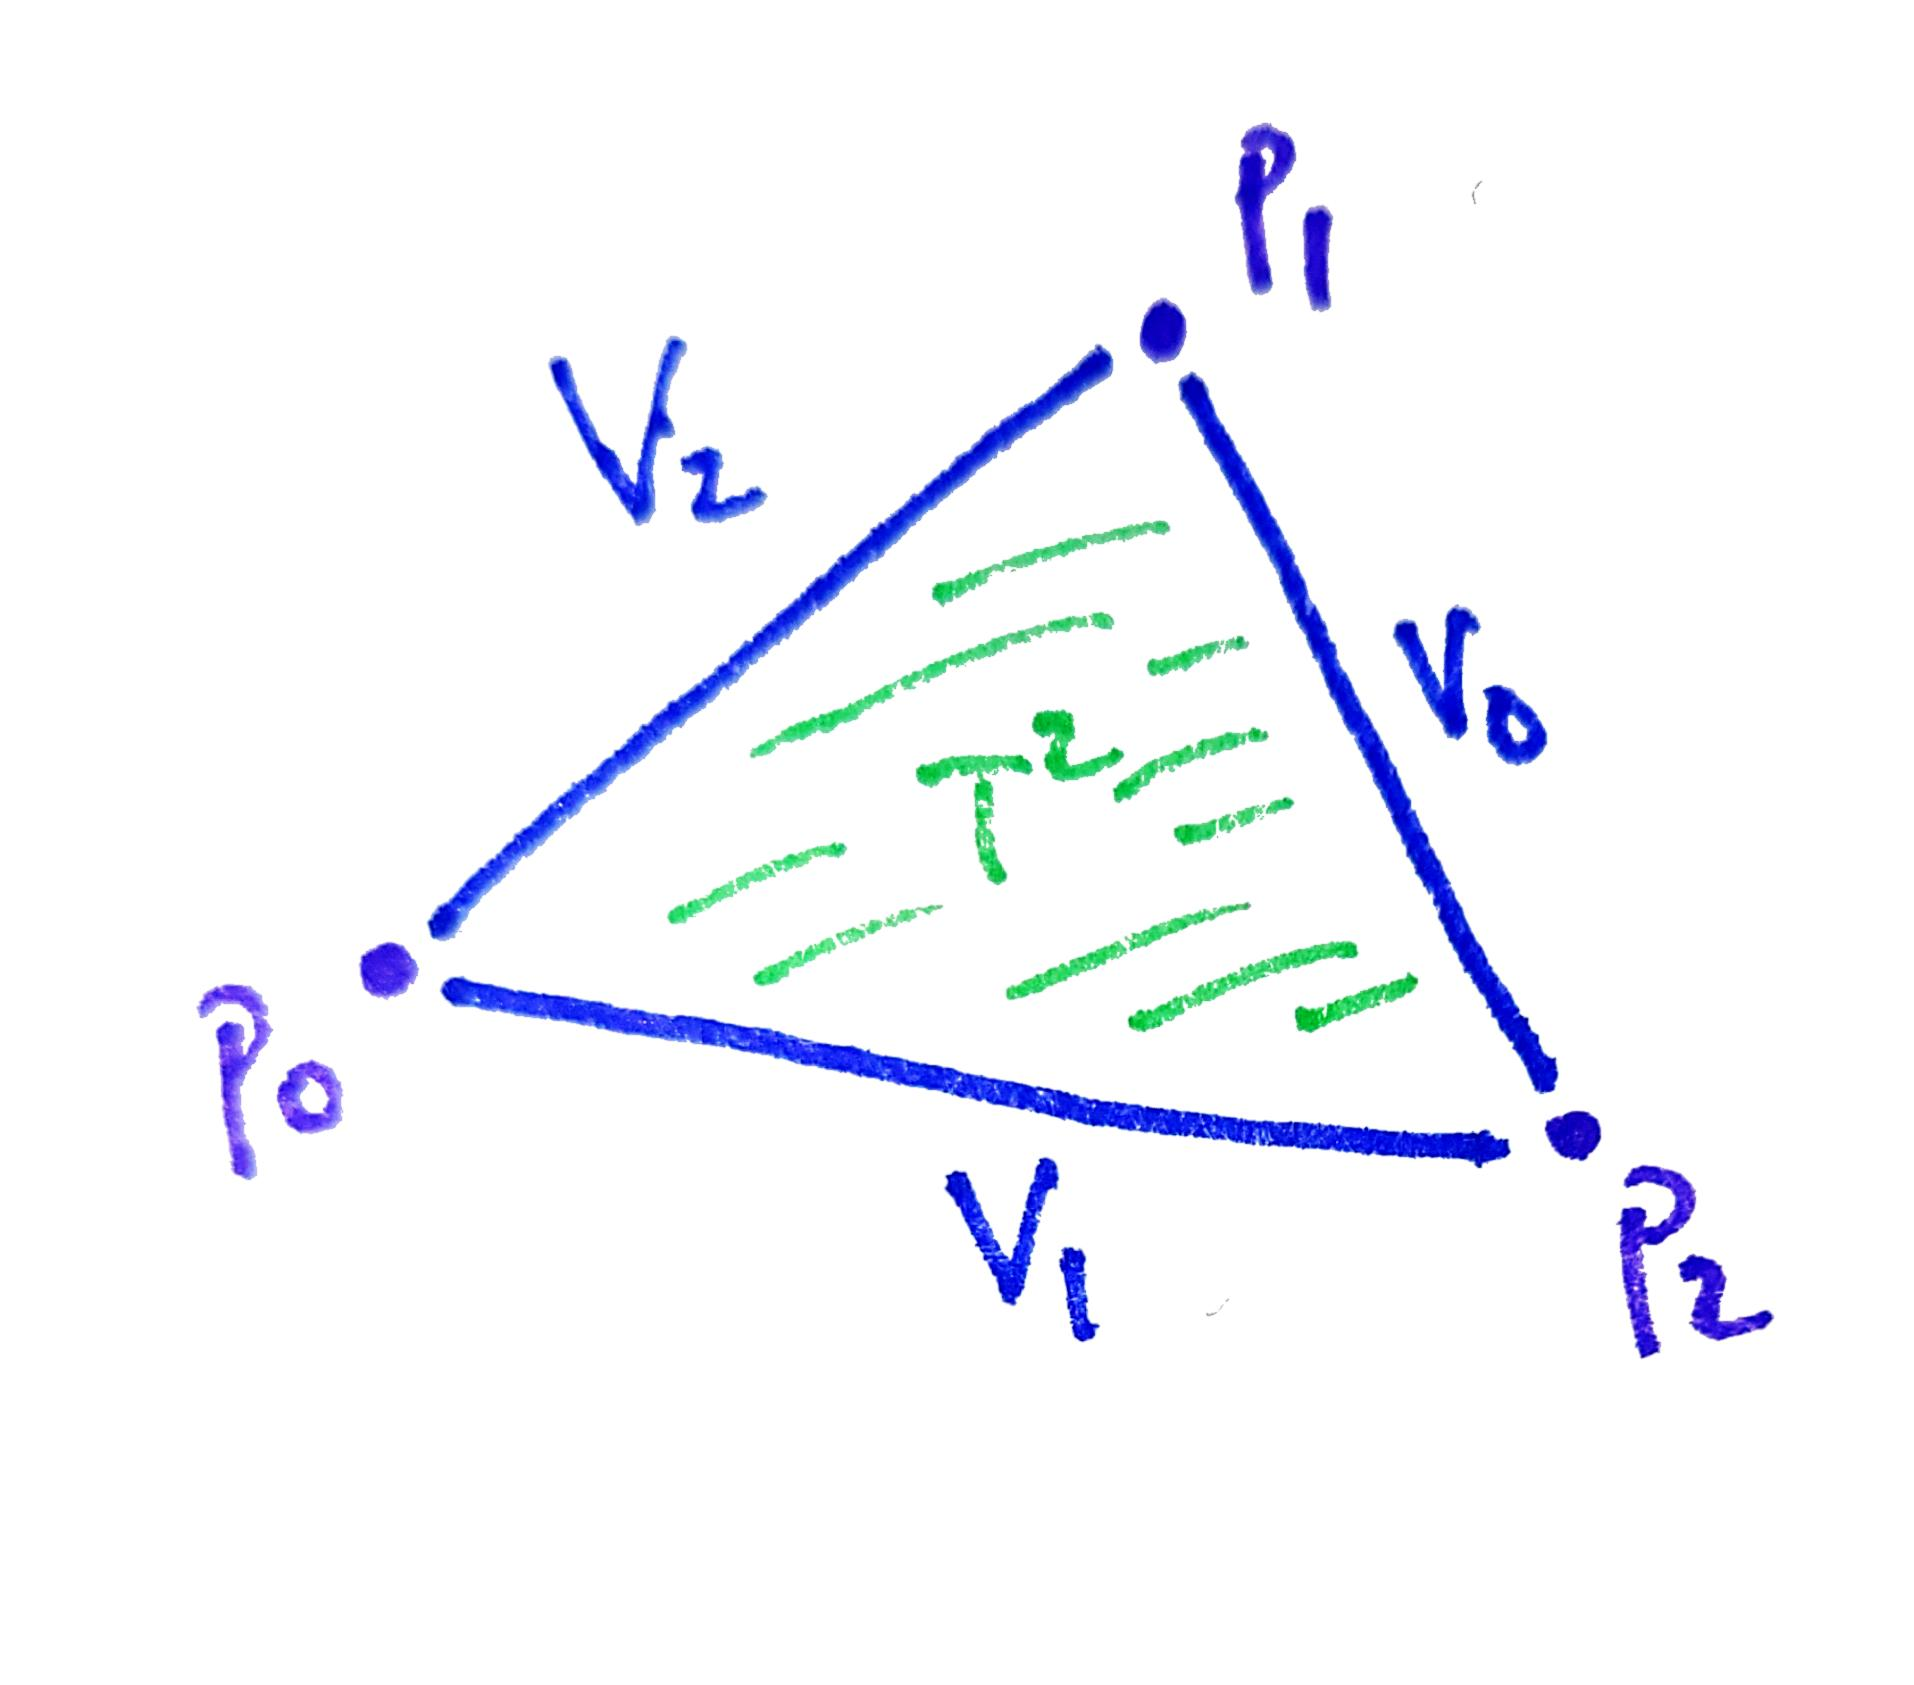
\includegraphics[scale=0.08]{diagrams/2024_01_18 21_02 Office Lens.jpg}
\end{center}
In particular, this gives us a stratification of \(\P^2\), with strata \(\T^2\), \(\C^* = T^1\) corresponding to \(V_i\) with the vertices removed, and the three vertices.

\printindex

\end{document}